\stopallthesefloats
\subsection{Cost of Cache Coherence}
\cite{Nowotsch2012LeveragingMC} places itself in a context similar to this
thesis: the issues of interference in multi-core architecture preventing their
use in avionics. More precisely, the paper proposes an analysis of an
architecture through benchmarks to ensure that tasks running in parallel can
correctly be time partitioned. The tasks in question involve mixed-criticality,
meaning that some tasks are more important than others, and thus lower
importance tasks must not impede higher importance ones.

The studied architecture is a NXP QorIQ P4080, featuring eight single-thread
cores with their own L1 and L2 caches, and interconnected through a CoreNet
Fabric implementing the MESI cache coherence protocol. There are also two L3
caches accessible through the interconnect.

The main sources of interference studied in \cite{Nowotsch2012LeveragingMC} are
simultaneous accesses to the interconnect and the main memory, as well as the
latencies induced by cache coherence. The idea is to have one core act as the
active observer, meaning that it is where time is measured, but it also performs
some operation. The other cores only act as a source of interference, and
multiple benchmarks are performed to see how increasing the number of secondary
cores influences the time measured by the observer core. This is similar to the
approaches presented in the previous section, with the difference being that
instead of targetting a specific component, the benchmarks are solely focused on
memory access, and the comparison is made on cores performing either
\textit{read} or \textit{write} on memory elements.

For the evaluation of the latencies induced by cache coherence, three categories
of cache coherence benchmarks are considered:
\begin{itemize}
\item \textbf{disabled:} No cache coherence enabled (i.e.~the baseline), where
its mechanisms are disabled and the cores do not target any of the same memory
elements.
\item \textbf{static:} Cache coherence mechanisms are enabled, but the cores
still do not target any of the same memory elements.
\item \textbf{dynamic:} Cache coherence enabled, and cores only target shared
memory elements.
\end{itemize}
This is made possible by the fact that the architecture supports disabling cache
coherence all together. For all three categories, sub-benchmarks are performed,
in which the observer core either reads or writes memory elements while the
secondary core also perform either reading or writing (thus resulting in four
combinations for each category of cache coherence: read read - \textit{rr}, read
- write, \textit{rw}, \textit{wr}, and \textit{ww}).

\begin{figure}[hbt!]
\lstinputlisting{\chapterdirectory/figure/micro_bench/06214768_code.txt}
\caption{%
Algorithm overview for \cite{Nowotsch2012LeveragingMC} (taken from the paper)
}
\label{fig:micro_bench:cache_coherence_avionics_algo}
\end{figure}

Figure~\ref{fig:micro_bench:cache_coherence_avionics_algo} shows the algorithm
used by \cite{10.1109/PACT.2009.22}. Prior to each measurement, the caches are
flushed, then the cores synchronize with each other. Time is recorder using
utilities from the cores, which avoids making \lstinline!time()! be a source of
interference. The measured operation takes three parameters:
\lstinline!OPERATION! corresponds to either reading or writing,
\lstinline!NBYTES! is the number of bytes accessed in a measurement,
\lstinline!GAP! is the distance between the accesses made in order to target
separate cache lines and thus ensure that all accesses are cache misses. The
number of measures is controlled by \lstinline!NMEAS!. The
\lstinline!__asm_write_loop_gap64! corresponds to a \lstinline!meas_loop! for
a writing operation with a gap of 64 bytes.

\begin{figure}[hbt!]
\begin{center}
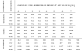
\includegraphics[width=0.7\textwidth]{\chapterdirectory/figure/micro_bench/cache_coherence_avionics.pdf}
\end{center}
\caption{Observed execution times depending on cache coherence and number of
active cores (adapted from \cite{Nowotsch2012LeveragingMC})}%
\label{fig:micro_bench:cache_coherence_avionics}
\end{figure}

The results of these benchmarks are shown in
Figure~\ref{fig:micro_bench:cache_coherence_avionics}.
\paragraph{Comparing \textit{Disabled} and \textit{Static} Cache Coherence:}
\textit{Static} cache coherence (mechanisms enabled, but each core access
different memory elements) does have an overhead compared to no cache
coherence at all when performing read operations, regardless of the operation
being performed by the other cores. For writing, this overhead is much lower.
This is interesting, as the \textit{static} benchmarks are the same experiment
as the \textit{disabled} cache coherence, meaning that effectively measures the
minimal overhead induced by having cache coherence mechanisms active,
regardless of how their are used. Thus, even when not having any use for it,
keeping cache coherence mechanisms enabled does lead to a increase in execution times.
This makes an argument for taking extra steps and disabling cache coherence for
memory elements that are not shared.

\paragraph{Comparing \textit{Static} and \textit{Dynamic} Cache Coherence:}
\textit{Dynamic} cache coherence (cache coherence enabled, and accesses
made to only shared memory elements) leads to the reverse: read operations yield
better execution time compared to writes. The best execution times are obtained by reading
while the other cores write, and the worst by writing while other cores are
writing as well. This is a surprising result (\textit{wr} and \textit{ww} being
slower than \textit{rr} and \textit{rw}), but these benchmarks do not take
coherence state of memory elements into account. The order in which cores get to
perform their operation changes that coherence state, and thus it changes the
cache's response  to other cores' operations, which in turn changes the execution time
results. Because of this, the results for \textit{dynamic} cache coherence
analysis cannot be exploited for a precise measurement of the effects of cache
coherence on running software.

To summarize, \cite{Nowotsch2012LeveragingMC} does provide an interesting
metric, which is found by comparing the execution time between the \textit{disabled}
and \textit{static} benchmarks. The overhead caused by unrequited cache
coherence queries are considered to be a form of interference.  Indeed, this
corresponds to the \textit{minor} interference of
Chapter~\ref{chap:exposing_interference} (see
Definition~\ref{def:interference:minor}).

The lack of information on coherence states prevent the \textit{dynamic}
benchmarks from being reused in the context of this thesis. However, a more
appropriate form of benchmarking for cache coherence mechanisms with shared
memory elements is explored in the next section.

\stopallthesefloats
